% \appendix
\section{Recommendation for applying defect control at sharp tolerances}
\label{section:HBs_higher_tol}
\subsection{The Vshaped graph and dependence on unit weight parameters}
\label{section:v_shaped_graph}
As we have shown several times in this thesis, the maximum order of accuracy of an interpolant depends on the value of the parameter $\alpha$ for the HB6 case and $\alpha$ and $\beta$ in the HB8 case. Furthermore, the accuracy also follows a V-shape as the interpolation error for sufficiently small $h$ reaches the round-off error. This is because the derivative of the interpolant uses a term in O($\frac{1}{h})$ where $h$ is the step-size. In this section we will look into how much these issues affect our interpolation. 

\paragraph{HB4}
In HB4, the error across several problems, across several sampling points, and at different step-sizes is as shown in Figure $\ref{fig:v_shape_across_problems_hb4}$. We note that this is without any parameters and at each h and each point $x$, we sampled at $x$ and $x + h$ to create the interpolant. The scheme suffers from an $O(\frac{1}{h})$ rounding off error inherently.
\begin{figure}[H]
\centering
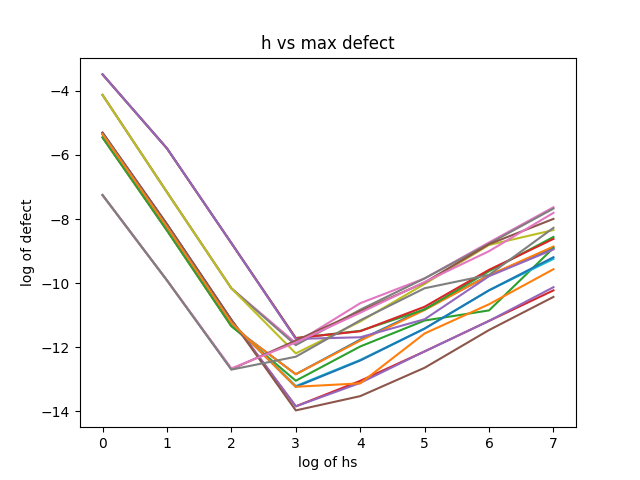
\includegraphics[width=0.7\linewidth]{./figures/v_shape_across_problems_hb4}
\caption{V-shape of HB4 across problems at several sampling points and with h}
\label{fig:v_shape_across_problems_hb4}
\end{figure}

We note that there is a clear optimal $h$ at about $10^{-3}$ and that we are able to achieve a tolerance of  $10^{-14}$ with some problems and $10^{-12}$ with almost every other problem. This gives us hope that this scheme can be used at very sharp tolerances. In this section, we will try several techniques to improve the situation. 


\paragraph{HB6}
In HB6, the error across several problems, across several sampling points, and at different step-sizes is as shown in Figure $\ref{fig:v_shape_across_problems_hb6}$. We note that that the parameter $\alpha$ is constant at 1 throughout the whole process as we sample at the point, $x$ and the points $x+h$ and $x-h$. This is the ideal case as the interpolation error is thus minimised.

\begin{figure}[H]
\centering
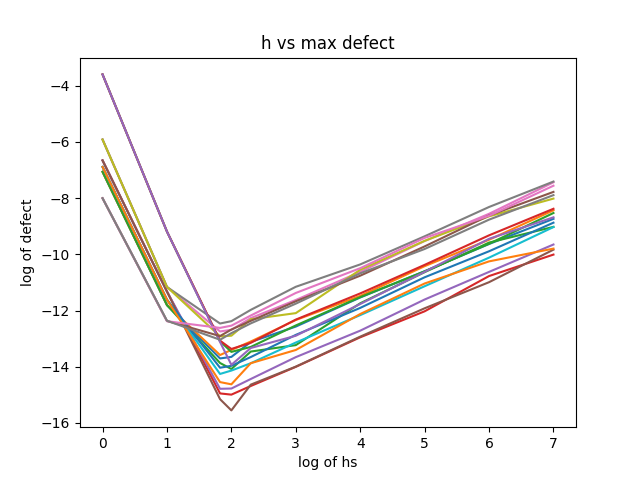
\includegraphics[width=0.7\linewidth]{./figures/v_shape_across_problems_hb6}
\caption{V-shape of HB6 across problems at several sampling points and with h}
\label{fig:v_shape_across_problems_hb6}
\end{figure}

We note that $\alpha$ was kept at 1 in Figure $\ref{fig:v_shape_across_problems_hb6}$. To see how the parameter $\alpha$ reduces the accuracy as it deviates from 1, see Figure $\ref{fig:hb6_alpha_v_shape}$.

We can see that the optimal $h$ is at around $10^{-2}$. We note that in most cases we were able to reach an error of $10^{-14}$ but in some cases we were only able to solve at $10^{-12}$. 


\paragraph{HB8}
In HB8, the error across several problems, across several sampling points, and at different step-sizes is as shown in Figure $\ref{fig:v_shape_across_problems_hb8}$. We note that that both parameters $\alpha$ and $\beta$ were constant at 1 throughout the whole process as we sample at the point, $x$ and the points $x+h$, $x-h$ and $x-2h$. This is the ideal case as the interpolation error is thus minimised. 

\begin{figure}[H]
\centering
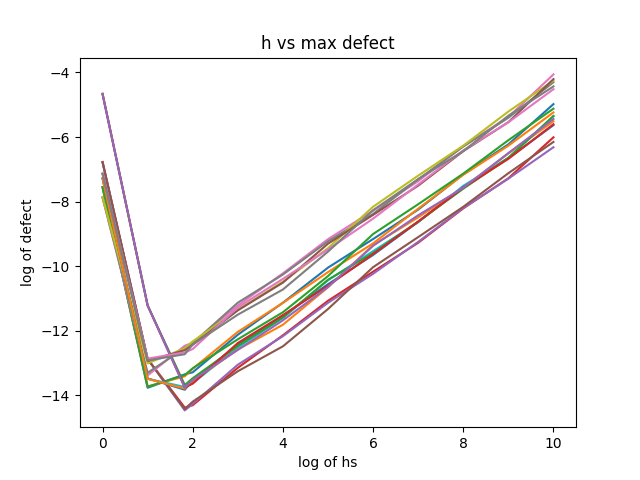
\includegraphics[width=0.7\linewidth]{./figures/v_shape_across_problems_hb8}
\caption{V-shape of HB8 across problems at several sampling points and with h}
\label{fig:v_shape_across_problems_hb8}
\end{figure}

We note that both $\alpha$ and $\beta$ were kept at 1 in Figure $\ref{fig:v_shape_across_problems_hb8}$. To see how the parameters $\alpha$ and $\beta$ reduces the accuracy as it deviates from 1, see Figure $\ref{fig:hb8_second_scheme_alpha_beta_test}$.

We can see that the optimal $h$ is at around $10^{-1}$ and $10^{-2}$. We note that in most cases we were able to reach an error of $10^{-14}$ but in some cases we were only able to solve at $10^{-13}$. 

\subsection{Horner's and Barycentric interpolants to get to lower tolerances.}
\label{section:horner_bary_forms}
We note that up to this form, we have been using the monomial form of each of the cubic, quintic and septic polynomials that we have derived. In the previous section, we have shown how these were suffering from being eventually dominated by the rounding-off error as we use smaller and smaller step-sizes. One idea to deal with the loss of accuracy due to the interference from the rounding-off error is to use a different representation of the polynomials. 

One idea is to use the Horner's form of the polynomials. The Horner's form of a polynomial minimises the number of multiplications that need to be undertaken during the evaluation. It is faster and also a less prone to rounding-off errors since fewer arithmetic operations are involved.

Another idea is to use a Barycentric interpolant. At the time of the creation of the interpolant, if it is of order $n$ over the interval $[a, b]$, we can find $n$ Chebyshev points in the interval and then sample the interpolant at these $n$ points and then fit a Barycentric interpolant to these data points. A Barycentric interpolant using $n$ data points is of order $n$ and if such an interpolant is used to interpolate a polynomial of order $n$, it perfectly matches the polynomial that is, this process gives a different but exact representation of the original polynomial. The Chebyshev points are used to guarantee the minimum interpolation error.

We will use these two interpolation schemes to supplement the Hermite Birkhoff interpolants HB4, HB6 and HB8 at a few different sampling points at different problems and report on the improvements that they give.

\begin{figure}[H]
\centering
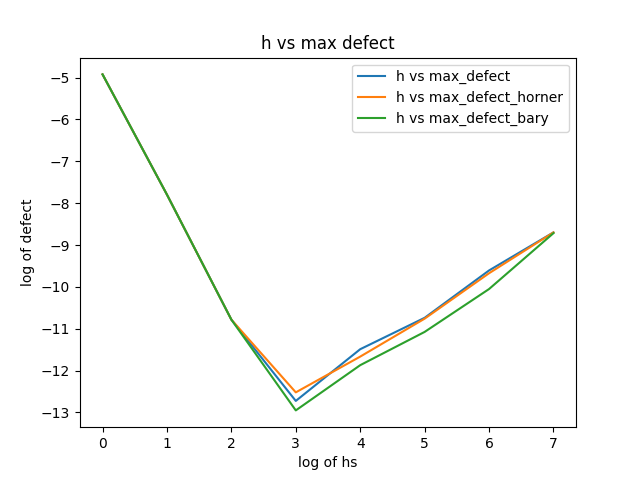
\includegraphics[width=0.7\linewidth]{./figures/typical_interp_horner_bary_hb4}
\caption{Typical plot of the HB4 interpolant monomial form vs the Horner form vs the Barycentric form}
\label{fig:typical_interp_horner_bary_hb4}
\end{figure}

Figure $\ref{fig:typical_interp_horner_bary_hb4}$ shows a typical plot of HB4 in the monomial form alongside its Horner form and Barycentric interpolation forms. We can report that the Horner form almost always matches the accuracy of the interpolant but that the Barycentric form slightly improves the accuracy. The V-shape is inevitable as both forms either themselves suffer from $O(\frac{1}{h})$ rounding-off error or interpolate over an interpolant that suffers from such a rounding-off error.

\begin{figure}[H]
\centering
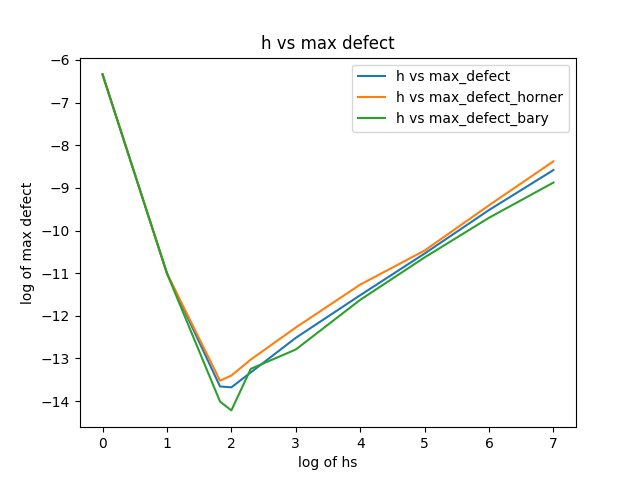
\includegraphics[width=0.7\linewidth]{./figures/typical_interp_horner_bary_hb6}
\caption{Typical plot of the HB6 interpolant monomial form vs the Horner form vs the Barycentric form}
\label{fig:typical_interp_horner_bary_hb6}
\end{figure}

Figure $\ref{fig:typical_interp_horner_bary_hb6}$ shows a typical plot of HB6 in the monomial form alongside its Horner form and Barycentric interpolation forms. We note that the parameter $\alpha$ is kept at 1 in the above plot. We can report that the Horner form almost always matches the accuracy of the interpolant but that the Barycentric form slightly improves the accuracy. The V-shape is inevitable as both forms either themselves suffer from $O(\frac{1}{h})$ rounding-off error or interpolate over an interpolant that suffers from such a rounding-off error.

\begin{figure}[H]
\centering
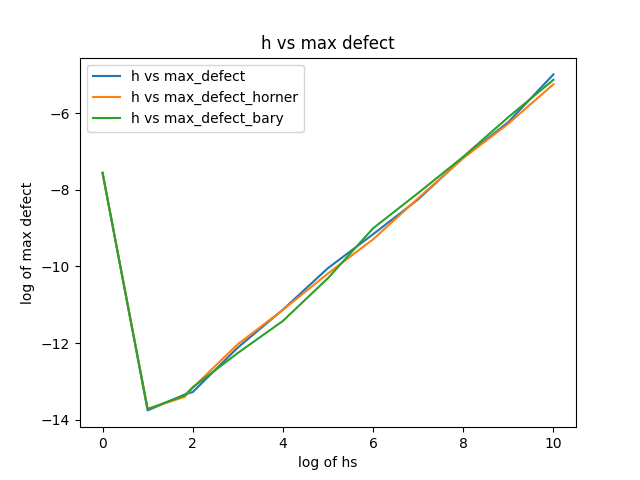
\includegraphics[width=0.7\linewidth]{./figures/typical_interp_horner_bary_hb8}
\caption{Typical plot of the HB8 interpolant monomial form vs the Horner form vs the Barycentric form}
\label{fig:typical_interp_horner_bary_hb8}
\end{figure}

Figure $\ref{fig:typical_interp_horner_bary_hb8}$ shows the typical plot of HB6 in the monomial form alongside its Horner form and Barycentric interpolation forms. We note that the parameters $\alpha$ and $\beta$ are kept at 1 in the above plot. For the case of HB8, the use of the Horner method or even the Barycentric method does not improve the situation. The monomial form is as accurate as we can get. The V-shape is inevitable as both forms either themselves suffer from $O(\frac{1}{h})$ rounding-off error or interpolate over an interpolant that suffers from such a rounding-off error.

\subsection{Solving at sharp tolerances}
\label{section:solving_at_sharp_tolerances}
Using the recommendations, we show that the scheme can be used at very sharp tolerances for RK4 with HB6 and RK6 with HB8. In the plots below, we do not employ the switch from variable parameters to static parameters as they are not needed. The first few steps are all necessarily small and thus do not go out of range. The initial $h$ value is the experimental optimal $h$ value and we use the static parameters solvers. 

\subsubsection{RK4 with HB6}
\paragraph{Problem 1 results}
Figures $\ref{fig:sharp_tolerance_rk4_with_hb6_p1_global_defect}$, $\ref{fig:sharp_tolerance_rk4_with_hb6_p1_global_error}$ and $\ref{fig:sharp_tolerance_rk4_with_hb6_p1_scaled_defects}$ shows the results of using RK4 with HB6 and some of the recommendations on Problem 1. We note that an absolute tolerance of $2.5 \times 10^{-12}$ is applied on the maximum defect within the step and this can be shown to occur at $0.2h$ and $0.8h$ along a step of size, h. See Figure $\ref{fig:sharp_tolerance_rk4_with_hb6_p1_scaled_defects}$, to see the scaled defect reaching a maximum near these points. We note that we are able to successfully control the defect of the continuous numerical solution using this approach, see Figure $\ref{fig:sharp_tolerance_rk4_with_hb6_p1_global_defect}$. 

\begin{figure}[H]
\centering
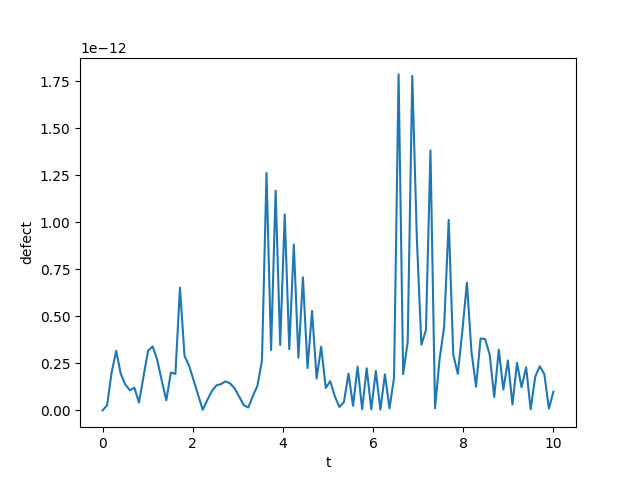
\includegraphics[width=0.7\linewidth]{./figures/sharp_tolerance_rk4_with_hb6_p1_global_defect}
\caption{Defect across entire domain for RK4 with HB6 using $\alpha = 1$ and optimal h as the starting h value on problem 1 at an absolute tolerance of $2.5 \times 10^{-12}$.}
\label{fig:sharp_tolerance_rk4_with_hb6_p1_global_defect}
\end{figure}

\begin{figure}[H]
\centering
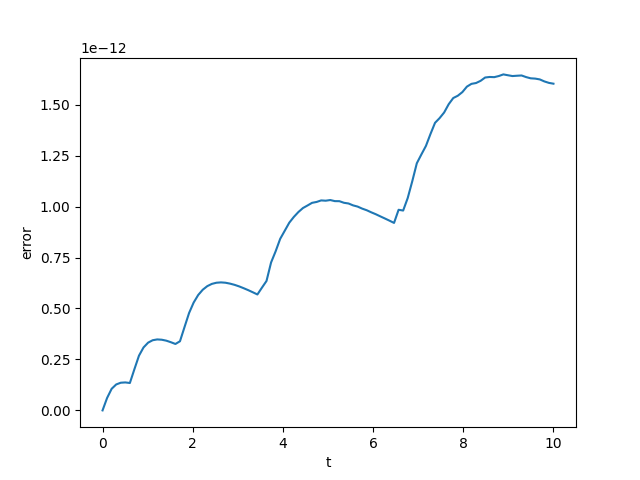
\includegraphics[width=0.7\linewidth]{./figures/sharp_tolerance_rk4_with_hb6_p1_global_error}
\caption{Global Error for RK4 with HB6 using $\alpha = 1$ and optimal h as the starting h value on problem 1 at an absolute tolerance of $2.5 \times 10^{-12}$.}
\label{fig:sharp_tolerance_rk4_with_hb6_p1_global_error}
\end{figure}

\begin{figure}[H]
\centering
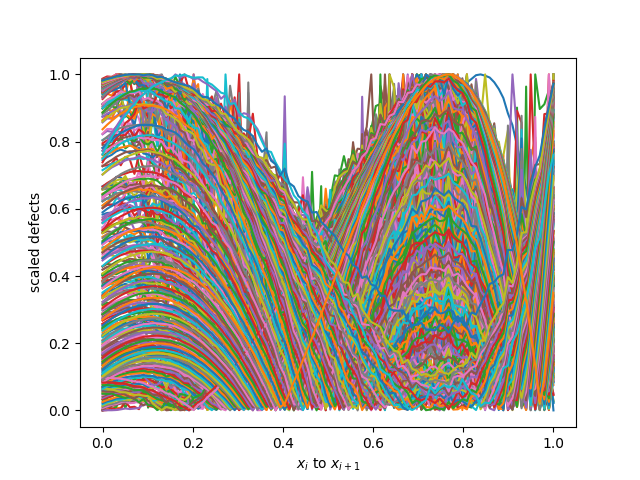
\includegraphics[width=0.7\linewidth]{./figures/sharp_tolerance_rk4_with_hb6_p1_scaled_defects}
\caption{Scaled Defects for RK4 with HB6 using $\alpha = 1$ and optimal h as the starting h value on problem 1 at an absolute tolerance of $2.5 \times 10^{-12}$ mapped onto $[0, 1]$.}
\label{fig:sharp_tolerance_rk4_with_hb6_p1_scaled_defects}
\end{figure}

\paragraph{Problem 2 results}
Figures $\ref{fig:sharp_tolerance_rk4_with_hb6_p2_global_defect}$, $\ref{fig:sharp_tolerance_rk4_with_hb6_p2_global_error}$ and $\ref{fig:sharp_tolerance_rk4_with_hb6_p2_scaled_defects}$ shows the results of using RK4 with HB6 and some of the recommendations on Problem 2. We note that an absolute tolerance of $2.5 \times 10^{-12}$ is applied on the maximum defect within the step and this can be shown to occur at $0.8h$ along a step of size, h. See Figure $\ref{fig:sharp_tolerance_rk4_with_hb6_p2_scaled_defects}$, to see the scaled defect reaching a maximum near these points. We note that we are able to successfully control the defect of the continuous numerical solution using this approach, see Figure $\ref{fig:sharp_tolerance_rk4_with_hb6_p2_global_defect}$. 

\begin{figure}[H]
\centering
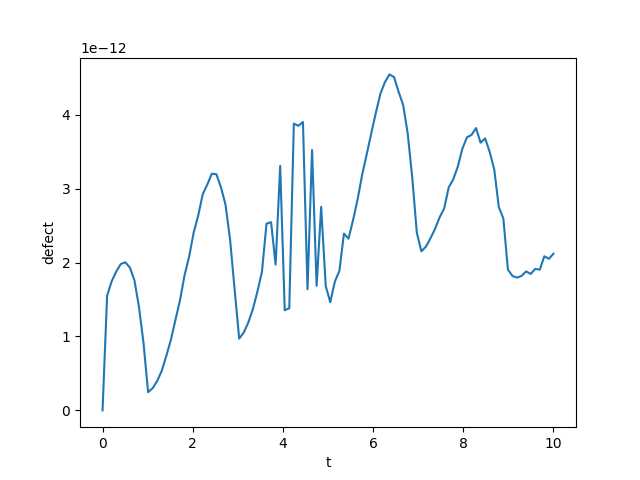
\includegraphics[width=0.7\linewidth]{./figures/sharp_tolerance_rk4_with_hb6_p2_global_defect}
\caption{Defect across entire domain for RK4 with HB6 using $\alpha = 1$ and optimal h as the starting h value on problem 2 at an absolute tolerance of $2.5 \times 10^{-12}$.}
\label{fig:sharp_tolerance_rk4_with_hb6_p2_global_defect}
\end{figure}

\begin{figure}[H]
\centering
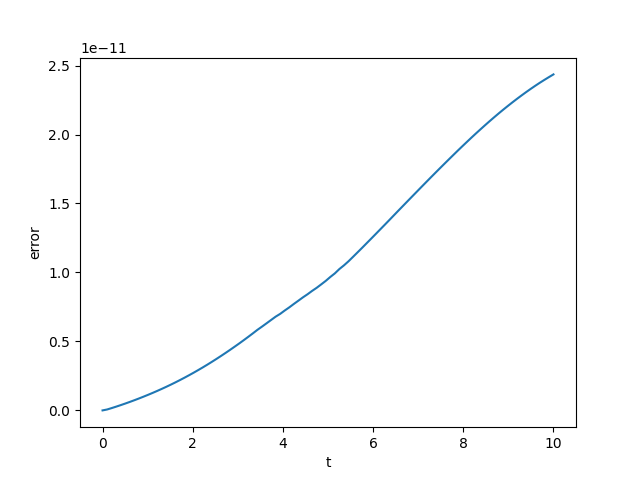
\includegraphics[width=0.7\linewidth]{./figures/sharp_tolerance_rk4_with_hb6_p2_global_error}
\caption{Global Error of RK4 with HB6 using $\alpha = 1$ and optimal h as the starting h value on problem 2 at an absolute tolerance of $2.5 \times 10^{-12}$.}
\label{fig:sharp_tolerance_rk4_with_hb6_p2_global_error}
\end{figure}

\begin{figure}[H]
\centering
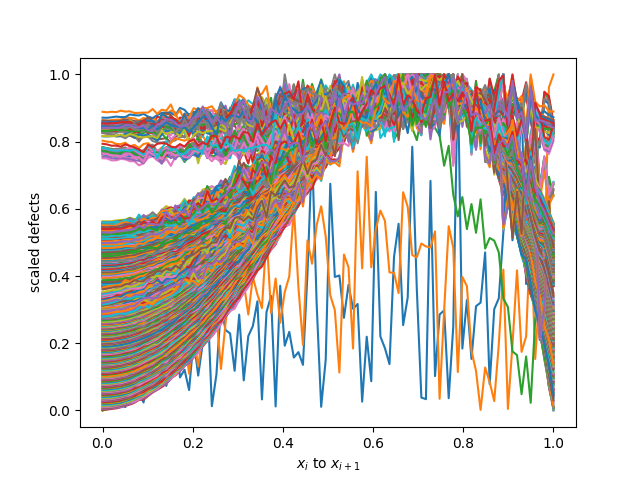
\includegraphics[width=0.7\linewidth]{./figures/sharp_tolerance_rk4_with_hb6_p2_scaled_defects}
\caption{Scaled Defects of RK4 with HB6 using $\alpha = 1$ and optimal h as the starting h value on problem 2 at an absolute tolerance of $2.5 \times 10^{-12}$ mapped onto $[0, 1]$.}
\label{fig:sharp_tolerance_rk4_with_hb6_p2_scaled_defects}
\end{figure}

\paragraph{Problem 3 results}
Figures $\ref{fig:sharp_tolerance_rk4_with_hb6_p3_global_defect}$, $\ref{fig:sharp_tolerance_rk4_with_hb6_p3_global_error}$ and $\ref{fig:sharp_tolerance_rk4_with_hb6_p3_scaled_defects}$ shows the results of using RK4 with HB6 and some of the recommendations on Problem 3. We note that an absolute tolerance of $2.5 \times 10^{-12}$ is applied on the maximum defect within the step and this can be shown to occur at $0.2h$ or $0.8h$ along a step of size, h. See Figure $\ref{fig:sharp_tolerance_rk4_with_hb6_p3_scaled_defects}$, to see the scaled defect reaching a maximum near these points. We note that we are able to successfully control the defect of the continuous numerical solution using this approach, see Figure $\ref{fig:sharp_tolerance_rk4_with_hb6_p3_global_defect}$. 


\begin{figure}[H]
\centering
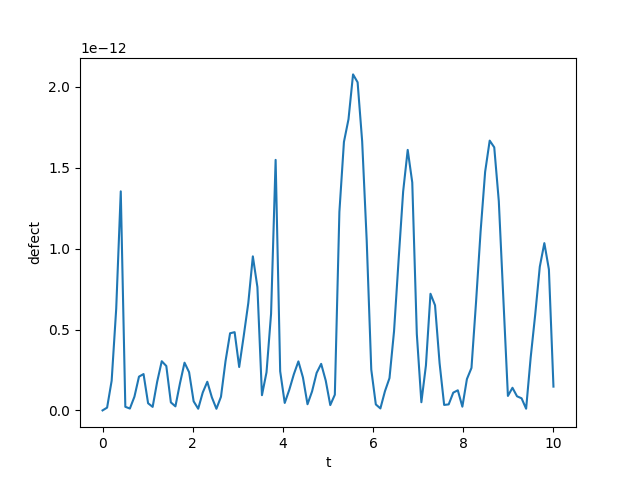
\includegraphics[width=0.7\linewidth]{./figures/sharp_tolerance_rk4_with_hb6_p3_global_defect}
\caption{Defect across entire domain for RK4 with HB6 using $\alpha = 1$ and optimal h as the starting h value on problem 3 at an absolute tolerance of $2.5 \times 10^{-12}$.}
\label{fig:sharp_tolerance_rk4_with_hb6_p3_global_defect}
\end{figure}

\begin{figure}[H]
\centering
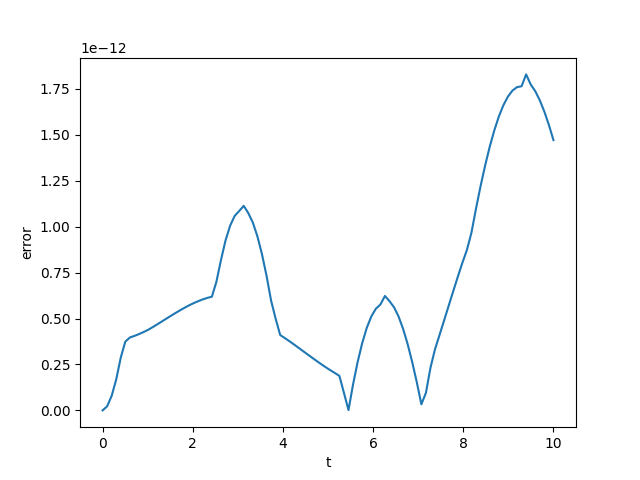
\includegraphics[width=0.7\linewidth]{./figures/sharp_tolerance_rk4_with_hb6_p3_global_error}
\caption{Global Error for RK4 with HB6 using $\alpha = 1$ and optimal h as the starting h value on problem 3 at an absolute tolerance of $2.5 \times 10^{-12}$.}
\label{fig:sharp_tolerance_rk4_with_hb6_p3_global_error}
\end{figure}

\begin{figure}[H]
\centering
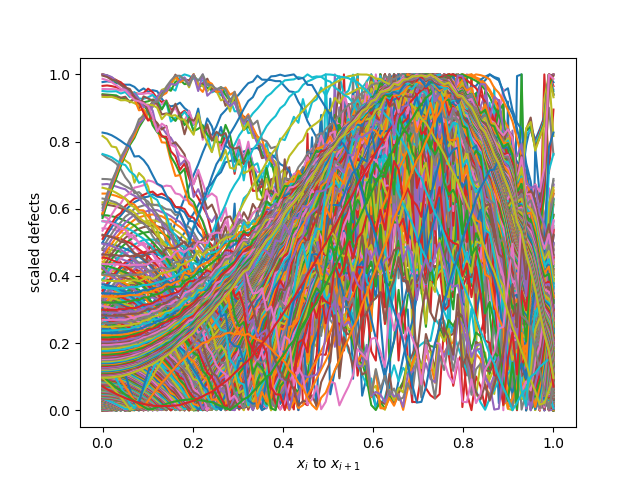
\includegraphics[width=0.7\linewidth]{./figures/sharp_tolerance_rk4_with_hb6_p3_scaled_defects}
\caption{Scaled Defects for RK4 with HB6 using alpha = 1 and optimal h as the starting h value on problem 3 at an absolute tolerance of $2.5 \times 10^{-12}$ mapped onto $[0, 1]$.}
\label{fig:sharp_tolerance_rk4_with_hb6_p3_scaled_defects}
\end{figure}

\begin{table}[h]
\caption {RK4 with HB6 using $\alpha = 1$ and optimal h as the starting h value at sharp tolerance} \label{tab:rk4_with_hb6_sharp_tolerance}
\begin{center}
\begin{tabular}{ c c c } 
Problem & n successful steps      &       nsteps \\ 
1       & 443                     &        523   \\ 
2       & 534                     &        568  \\
3       & 1378                    &        1731  \\
\end{tabular}
\end{center}
\end{table}	


\subsubsection{RK6 with HB8}

\paragraph{Problem 1 results}
Figures $\ref{fig:sharp_tolerance_rk6_with_hb8_p1_global_defect}$, $\ref{fig:sharp_tolerance_rk6_with_hb8_p1_global_error}$ and $\ref{fig:sharp_tolerance_rk6_with_hb8_p1_scaled_defects}$ shows the results of using RK6 with HB8 and some of the recommendations on Problem 1. We note that an absolute tolerance of $2.5 \times 10^{-12}$ is applied on the maximum defect within the step and this can be shown to occur at $0.2h$ or $0.8h$ along a step of size, h. See Figure $\ref{fig:sharp_tolerance_rk6_with_hb8_p1_scaled_defects}$, to see the scaled defect reaching a maximum near these points. We note that we are able to successfully control the defect of the continuous numerical solution using this approach, see Figure $\ref{fig:sharp_tolerance_rk6_with_hb8_p1_global_defect}$. 

\begin{figure}[H]
\centering
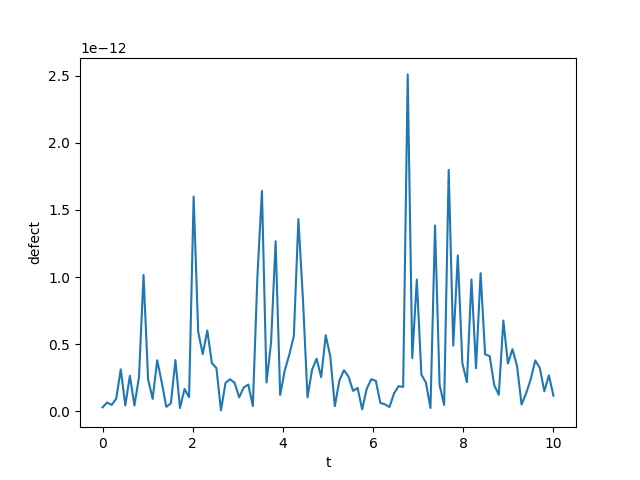
\includegraphics[width=0.7\linewidth]{./figures/sharp_tolerance_rk6_with_hb8_p1_global_defect}
\caption{Defect across entire domain for RK6 with HB8 using $\alpha$ and $\beta$ = 1 and optimal h as the starting h value on problem 1 at an absolute tolerance of $2.5 \times 10^{-12}$.}
\label{fig:sharp_tolerance_rk6_with_hb8_p1_global_defect}
\end{figure}

\begin{figure}[H]
\centering
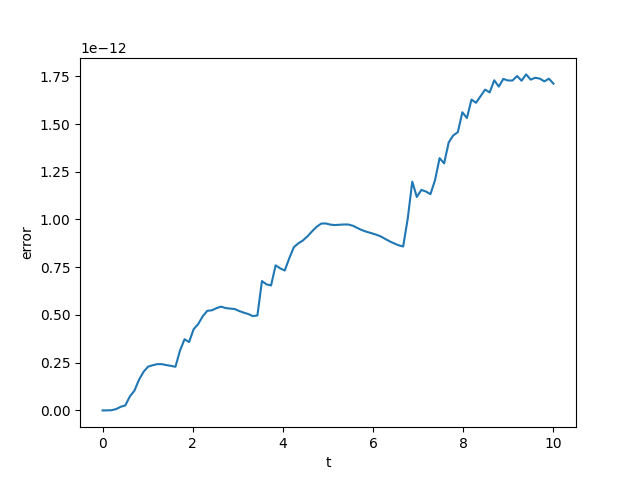
\includegraphics[width=0.7\linewidth]{./figures/sharp_tolerance_rk6_with_hb8_p1_global_error}
\caption{Global Error for RK6 with HB8 using $\alpha$ and $\beta$ = 1 and optimal h as the starting h value on problem 1 at an absolute tolerance of $2.5 \times 10^{-12}$.}
\label{fig:sharp_tolerance_rk6_with_hb8_p1_global_error}
\end{figure}

\begin{figure}[H]
\centering
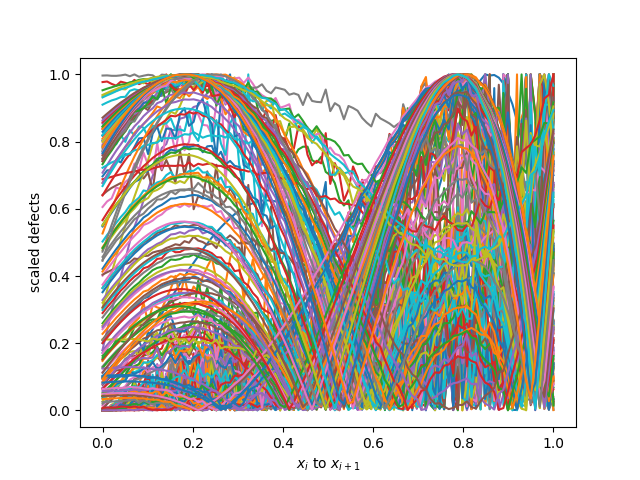
\includegraphics[width=0.7\linewidth]{./figures/sharp_tolerance_rk6_with_hb8_p1_scaled_defects}
\caption{Scaled Defects for RK6 with HB8 using $\alpha$ and $\beta$ = 1 and optimal h as the starting h value on problem 1 at an absolute tolerance of $2.5 \times 10^{-12}$ mapped onto $[0, 1]$.}
\label{fig:sharp_tolerance_rk6_with_hb8_p1_scaled_defects}
\end{figure}

\paragraph{Problem 2 results}
Figures $\ref{fig:sharp_tolerance_rk6_with_hb8_p2_global_defect}$, $\ref{fig:sharp_tolerance_rk6_with_hb8_p2_global_error}$ and $\ref{fig:sharp_tolerance_rk6_with_hb8_p2_scaled_defects}$ shows the results of using RK6 with HB8 and some of the recommendations on Problem 2. We note that an absolute tolerance of $2.5 \times 10^{-12}$ is applied on the maximum defect within the step and this can be shown to occur at $0.8h$ along a step of size, h. See Figure $\ref{fig:sharp_tolerance_rk6_with_hb8_p2_scaled_defects}$, to see the scaled defect reaching a maximum near these points. We note that we are able to successfully control the defect of the continuous numerical solution using this approach, see Figure $\ref{fig:sharp_tolerance_rk6_with_hb8_p2_global_defect}$. 
\begin{figure}[H]
\centering
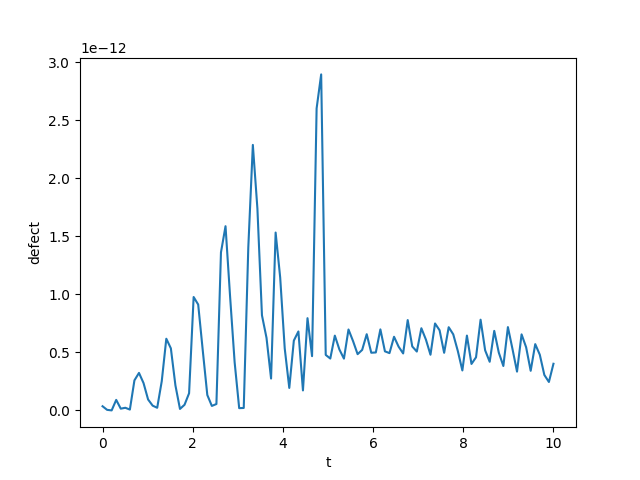
\includegraphics[width=0.7\linewidth]{./figures/sharp_tolerance_rk6_with_hb8_p2_global_defect}
\caption{Defect across entire domain for RK6 with HB8 using $\alpha$ and $\beta$ = 1 and optimal h as the starting h value on problem 2 at an absolute tolerance of $2.5 \times 10^{-12}$.}
\label{fig:sharp_tolerance_rk6_with_hb8_p2_global_defect}
\end{figure}

\begin{figure}[H]
\centering
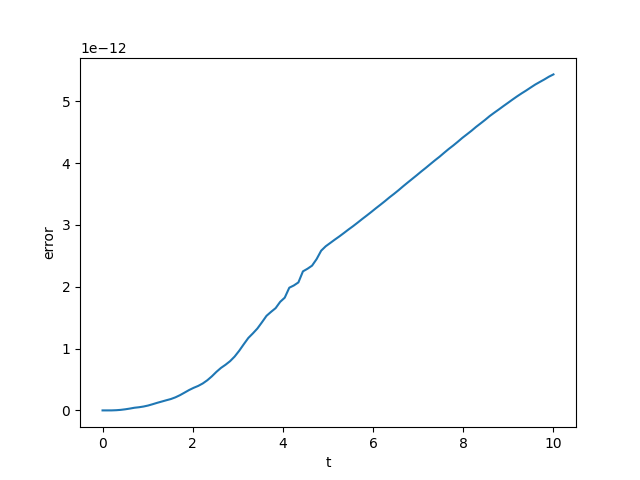
\includegraphics[width=0.7\linewidth]{./figures/sharp_tolerance_rk6_with_hb8_p2_global_error}
\caption{Global Error for RK6 with HB8 using $\alpha$ and $\beta$ = 1 and optimal h as the starting h value on problem 2 at an absolute tolerance of $2.5 \times 10^{-12}$.}
\label{fig:sharp_tolerance_rk6_with_hb8_p2_global_error}
\end{figure}

\begin{figure}[H]
\centering
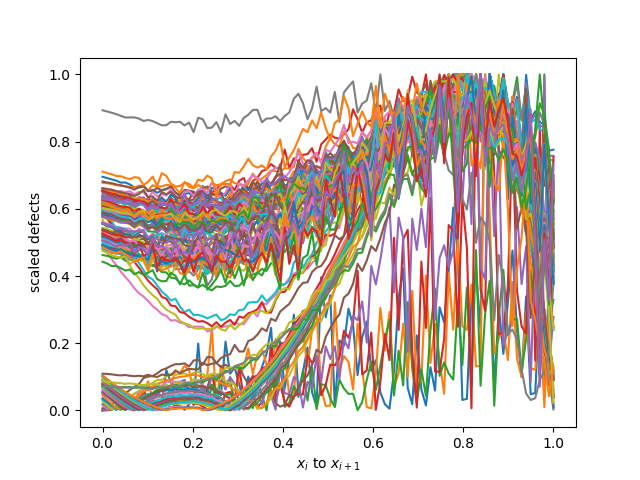
\includegraphics[width=0.7\linewidth]{./figures/sharp_tolerance_rk6_with_hb8_p2_scaled_defects}
\caption{Scaled Defects for RK6 with HB8 using $\alpha$ and $\beta$ = 1 and optimal h as the starting h value on problem 2 at an absolute tolerance of $2.5 \times 10^{-12}$ mapped onto $[0, 1]$.}
\label{fig:sharp_tolerance_rk6_with_hb8_p2_scaled_defects}
\end{figure}

\paragraph{Problem 3 results}
Figures $\ref{fig:sharp_tolerance_rk6_with_hb8_p3_global_defect}$, $\ref{fig:sharp_tolerance_rk6_with_hb8_p3_global_error}$ and $\ref{fig:sharp_tolerance_rk6_with_hb8_p3_scaled_defects}$ shows the results of using RK6 with HB8 and some of the recommendations on Problem 3. We note that an absolute tolerance of $2.5 \times 10^{-12}$ is applied on the maximum defect within the step and this can be shown to occur at $0.3h$ or $0.8h$ along a step of size, h. See Figure $\ref{fig:sharp_tolerance_rk6_with_hb8_p3_scaled_defects}$, to see the scaled defect reaching a maximum near these points. We note that we are able to successfully control the defect of the continuous numerical solution using this approach, see Figure $\ref{fig:sharp_tolerance_rk6_with_hb8_p3_global_defect}$. 
\begin{figure}[H]
\centering
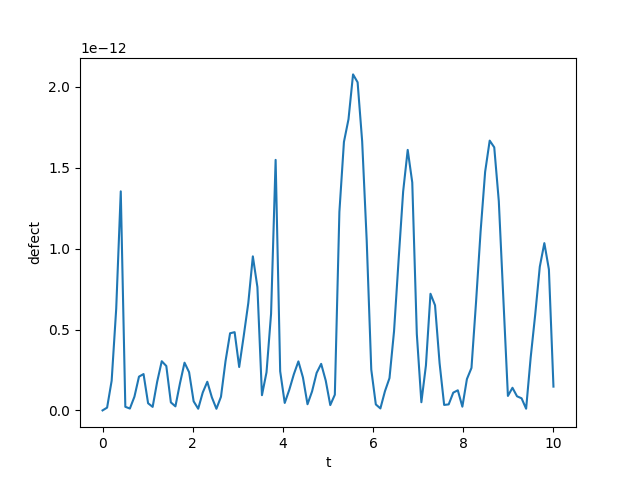
\includegraphics[width=0.7\linewidth]{./figures/sharp_tolerance_rk4_with_hb6_p3_global_defect}
\caption{Defect across entire domain for RK6 with HB8 using $\alpha$ and $\beta$ = 1 and optimal h as the starting h value on problem 3 at an absolute tolerance of $2.5 \times 10^{-12}$.}
\label{fig:sharp_tolerance_rk6_with_hb8_p3_global_defect}
\end{figure}

\begin{figure}[H]
\centering
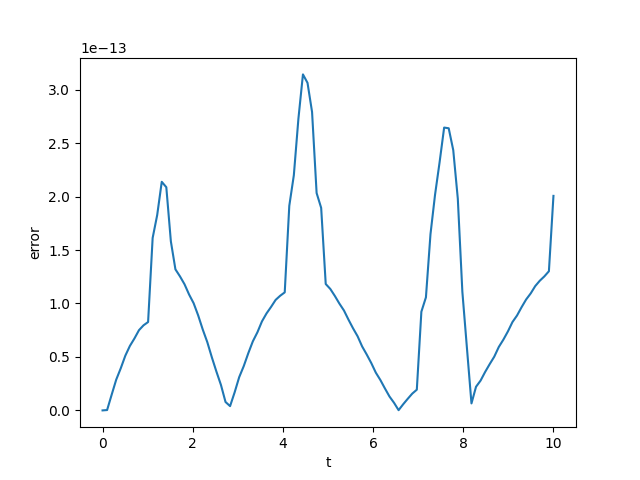
\includegraphics[width=0.7\linewidth]{./figures/sharp_tolerance_rk6_with_hb8_p3_global_error}
\caption{Global Error for RK6 with HB8 using $\alpha$ and $\beta$ = 1 and optimal h as the starting h value on problem 3 at an absolute tolerance of $2.5 \times 10^{-12}$.}
\label{fig:sharp_tolerance_rk6_with_hb8_p3_global_error}
\end{figure}

\begin{figure}[H]
\centering
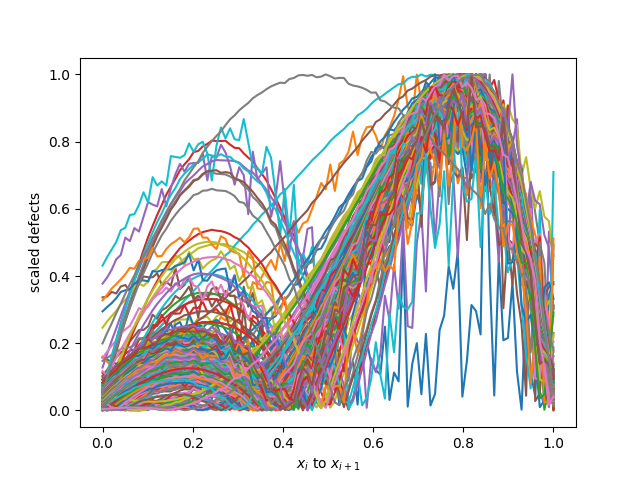
\includegraphics[width=0.7\linewidth]{./figures/sharp_tolerance_rk6_with_hb8_p3_scaled_defects}
\caption{Scaled Defects for RK6 with HB8 using $\alpha$ and $\beta$ = 1 and optimal h as the starting h value on problem 3 at an absolute tolerance of $2.5 \times 10^{-12}$ mapped onto $[0, 1]$.}
\label{fig:sharp_tolerance_rk6_with_hb8_p3_scaled_defects}
\end{figure}

\begin{table}[h]
\caption {rk6 with hb8 using static alpha and beta and optimal h as the starting h value at sharp tolerance} \label{tab:rk6_with_hb8_sharp_tolerance}
\begin{center}
\begin{tabular}{ c c c } 
Problem & n successful steps      &       nsteps    \\ 
1       & 261                     &        290      \\ 
2       & 134                     &        196      \\
3       & 297                     &        466      \\
\end{tabular}
\end{center}
\end{table}	
